\scanpage{27}
\uline{NB}
\[\chi_\infty(E)=\varepsilon(\mathbf R f_*(E))-\varepsilon(\mathbf R f_!(E))\]
Or on a vu que les deux $\varepsilon$ sont égaux, donc $\chi_\infty(E)=0$. De même on a
\[\delta_\infty(E)=\delta(\mathbf R f_*(E))\delta(\mathbf R f_!(E))^{-1}\]
et on a vu que
\[p^{(n+\rho)\chi(E)}\delta(\mathbf R f_*(E))^{-1}=\delta(\mathbf R f_!(E))\]
d'où
\[\left\{\begin{aligned}
\delta_\infty(E)&=p^{(n+\rho)\chi(E)}\delta(E)^{-2}=\varepsilon(E)^{-2}\quad\deleted{\unsure{\delta(E)^2p^{-(n+\rho)\chi(E)}}}\\
\varepsilon(E)&=\delta(E)p^{-(n+\rho)\chi(E)/2}
\end{aligned}\right.\]
\margin{($=\pm1$ si $X$ est \deleted{\unsure{complet}} propre)}
(qui est bien $1$ lorsque $X$ est complet !)

d'où l'équation fonctionnelle
\[\boxed{L_E^\infty\left(\frac1{p^{n+\rho}t}\right)L_E^\infty(t)\delta_\infty(E)=1}\]
\[\left(\delta_\infty(E)=p^{(n+\rho)\chi(E)}\delta(E)^{-2}\deleted{\unsure{\delta}}=\varepsilon(E)^{-2}\right)\]

[Invariants arithmétiques équivalents,

(moyennant la connaissance de l'invariant \uline{géométrique} $\chi(E)$, et de $q=\deleted{\unsure{p}}p^{n+\rho}$)
\margin{\fbox{\parbox{3.1cm}{\uline{NB}. $\varepsilon(E)=\pm1$ si $X$ complet}}}
\[\delta(E)=\delta_!^*(E),\quad\delta'(E)=\unsure{\delta_*^*(E)|\delta_\cdot^*(E)},\quad\varepsilon(E),\quad\delta_\infty(E)\]
]
\[\boxed{\delta(E)\delta'(E)=q^{\chi(E)}}\]
\[\boxed{\varepsilon(E)=\delta(E)q^{-\chi(E)/2}=\delta'(E)q^{-\chi(E)/2}}\]
\margin{\figure{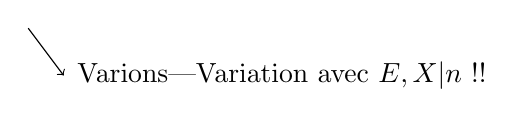
\begin{tikzpicture}[x=1cm,y=1cm]\draw[->] (0,0.6)--(0.45,0);\node[anchor=west] at (0.5,0) {\unsure{Varions|Variation} avec $E,\unsure{X|n}$ !!};\end{tikzpicture}}}
\[\boxed{\begin{aligned}
\delta_\infty(E)&=q^{\chi(E)}\delta(E)^{-2}=q^{-\chi(E)}\delta'(E)^{\unsure{2}}\\
&=\varepsilon(E)^{-2}
\end{aligned}}\]
\mspage{26}
